\documentclass[twoside]{book}

% Packages required by doxygen
\usepackage{fixltx2e}
\usepackage{calc}
\usepackage{doxygen}
\usepackage[export]{adjustbox} % also loads graphicx
\usepackage{graphicx}
\usepackage[utf8]{inputenc}
\usepackage{makeidx}
\usepackage{multicol}
\usepackage{multirow}
\PassOptionsToPackage{warn}{textcomp}
\usepackage{textcomp}
\usepackage[nointegrals]{wasysym}
\usepackage[table]{xcolor}

% Font selection
\usepackage[T1]{fontenc}
\usepackage[scaled=.90]{helvet}
\usepackage{courier}
\usepackage{amssymb}
\usepackage{sectsty}
\renewcommand{\familydefault}{\sfdefault}
\allsectionsfont{%
  \fontseries{bc}\selectfont%
  \color{darkgray}%
}
\renewcommand{\DoxyLabelFont}{%
  \fontseries{bc}\selectfont%
  \color{darkgray}%
}
\newcommand{\+}{\discretionary{\mbox{\scriptsize$\hookleftarrow$}}{}{}}

% Page & text layout
\usepackage{geometry}
\geometry{%
  a4paper,%
  top=2.5cm,%
  bottom=2.5cm,%
  left=2.5cm,%
  right=2.5cm%
}
\tolerance=750
\hfuzz=15pt
\hbadness=750
\setlength{\emergencystretch}{15pt}
\setlength{\parindent}{0cm}
\setlength{\parskip}{3ex plus 2ex minus 2ex}
\makeatletter
\renewcommand{\paragraph}{%
  \@startsection{paragraph}{4}{0ex}{-1.0ex}{1.0ex}{%
    \normalfont\normalsize\bfseries\SS@parafont%
  }%
}
\renewcommand{\subparagraph}{%
  \@startsection{subparagraph}{5}{0ex}{-1.0ex}{1.0ex}{%
    \normalfont\normalsize\bfseries\SS@subparafont%
  }%
}
\makeatother

% Headers & footers
\usepackage{fancyhdr}
\pagestyle{fancyplain}
\fancyhead[LE]{\fancyplain{}{\bfseries\thepage}}
\fancyhead[CE]{\fancyplain{}{}}
\fancyhead[RE]{\fancyplain{}{\bfseries\leftmark}}
\fancyhead[LO]{\fancyplain{}{\bfseries\rightmark}}
\fancyhead[CO]{\fancyplain{}{}}
\fancyhead[RO]{\fancyplain{}{\bfseries\thepage}}
\fancyfoot[LE]{\fancyplain{}{}}
\fancyfoot[CE]{\fancyplain{}{}}
\fancyfoot[RE]{\fancyplain{}{\bfseries\scriptsize Generated by Doxygen }}
\fancyfoot[LO]{\fancyplain{}{\bfseries\scriptsize Generated by Doxygen }}
\fancyfoot[CO]{\fancyplain{}{}}
\fancyfoot[RO]{\fancyplain{}{}}
\renewcommand{\footrulewidth}{0.4pt}
\renewcommand{\chaptermark}[1]{%
  \markboth{#1}{}%
}
\renewcommand{\sectionmark}[1]{%
  \markright{\thesection\ #1}%
}

% Indices & bibliography
\usepackage{natbib}
\usepackage[titles]{tocloft}
\setcounter{tocdepth}{3}
\setcounter{secnumdepth}{5}
\makeindex

% Hyperlinks (required, but should be loaded last)
\usepackage{ifpdf}
\ifpdf
  \usepackage[pdftex,pagebackref=true]{hyperref}
\else
  \usepackage[ps2pdf,pagebackref=true]{hyperref}
\fi
\hypersetup{%
  colorlinks=true,%
  linkcolor=blue,%
  citecolor=blue,%
  unicode%
}

% Custom commands
\newcommand{\clearemptydoublepage}{%
  \newpage{\pagestyle{empty}\cleardoublepage}%
}

\usepackage{caption}
\captionsetup{labelsep=space,justification=centering,font={bf},singlelinecheck=off,skip=4pt,position=top}

%===== C O N T E N T S =====

\begin{document}

% Titlepage & ToC
\hypersetup{pageanchor=false,
             bookmarksnumbered=true,
             pdfencoding=unicode
            }
\pagenumbering{alph}
\begin{titlepage}
\vspace*{7cm}
\begin{center}%
{\Large H\+P-\/\+A\+NN \\[1ex]\large 0.\+0.\+1 }\\
\vspace*{1cm}
{\large Generated by Doxygen 1.8.13}\\
\end{center}
\end{titlepage}
\clearemptydoublepage
\pagenumbering{roman}
\tableofcontents
\clearemptydoublepage
\pagenumbering{arabic}
\hypersetup{pageanchor=true}

%--- Begin generated contents ---
\chapter{Data Structure Index}
\section{Data Structures}
Here are the data structures with brief descriptions\+:\begin{DoxyCompactList}
\item\contentsline{section}{\hyperlink{structNeuron}{Neuron} \\*The basic structure of a \hyperlink{structNeuron}{Neuron} }{\pageref{structNeuron}}{}
\item\contentsline{section}{\hyperlink{structNeuronLayer}{Neuron\+Layer} \\*The basic structure of a neuron layer }{\pageref{structNeuronLayer}}{}
\end{DoxyCompactList}

\chapter{File Index}
\section{File List}
Here is a list of all documented files with brief descriptions\+:\begin{DoxyCompactList}
\item\contentsline{section}{/home/albert/\+Desktop/\+D\+E\+V/\+H\+P-\/\+A\+N\+N/include/\hyperlink{activation_8h}{activation.\+h} \\*This header file contains all the implemented activation functions and its derivatives }{\pageref{activation_8h}}{}
\item\contentsline{section}{/home/albert/\+Desktop/\+D\+E\+V/\+H\+P-\/\+A\+N\+N/include/\hyperlink{neuron_8h}{neuron.\+h} \\*This header file contains the structure of the \hyperlink{structNeuron}{Neuron} and its basic functions }{\pageref{neuron_8h}}{}
\item\contentsline{section}{/home/albert/\+Desktop/\+D\+E\+V/\+H\+P-\/\+A\+N\+N/include/\hyperlink{neuronLayer_8h}{neuron\+Layer.\+h} \\*This header file contains the structure of the \hyperlink{structNeuronLayer}{Neuron\+Layer} and its basic functions }{\pageref{neuronLayer_8h}}{}
\end{DoxyCompactList}

\chapter{Data Structure Documentation}
\hypertarget{structNeuron}{}\section{Neuron Struct Reference}
\label{structNeuron}\index{Neuron@{Neuron}}


The basic structure of a \hyperlink{structNeuron}{Neuron}.  




{\ttfamily \#include $<$neuron.\+h$>$}

\subsection*{Data Fields}
\begin{DoxyCompactItemize}
\item 
double \hyperlink{structNeuron_ac3093a71eb817e3b91ec4210707b0602}{val}
\item 
double \hyperlink{structNeuron_a11871bae6838438e083a6ecd2e611870}{act\+Val}
\end{DoxyCompactItemize}


\subsection{Detailed Description}
The basic structure of a \hyperlink{structNeuron}{Neuron}. 

\subsection{Field Documentation}
\mbox{\Hypertarget{structNeuron_a11871bae6838438e083a6ecd2e611870}\label{structNeuron_a11871bae6838438e083a6ecd2e611870}} 
\index{Neuron@{Neuron}!act\+Val@{act\+Val}}
\index{act\+Val@{act\+Val}!Neuron@{Neuron}}
\subsubsection{\texorpdfstring{act\+Val}{actVal}}
{\footnotesize\ttfamily double Neuron\+::act\+Val}

The activated value to send to the next neuron. \mbox{\Hypertarget{structNeuron_ac3093a71eb817e3b91ec4210707b0602}\label{structNeuron_ac3093a71eb817e3b91ec4210707b0602}} 
\index{Neuron@{Neuron}!val@{val}}
\index{val@{val}!Neuron@{Neuron}}
\subsubsection{\texorpdfstring{val}{val}}
{\footnotesize\ttfamily double Neuron\+::val}

The value that collects this neuron. 

The documentation for this struct was generated from the following file\+:\begin{DoxyCompactItemize}
\item 
/home/albert/\+Desktop/\+D\+E\+V/\+H\+P-\/\+A\+N\+N/include/\hyperlink{neuron_8h}{neuron.\+h}\end{DoxyCompactItemize}

\hypertarget{structNeuronLayer}{}\section{Neuron\+Layer Struct Reference}
\label{structNeuronLayer}\index{Neuron\+Layer@{Neuron\+Layer}}


The basic structure of a neuron layer.  




{\ttfamily \#include $<$neuron\+Layer.\+h$>$}



Collaboration diagram for Neuron\+Layer\+:\nopagebreak
\begin{figure}[H]
\begin{center}
\leavevmode
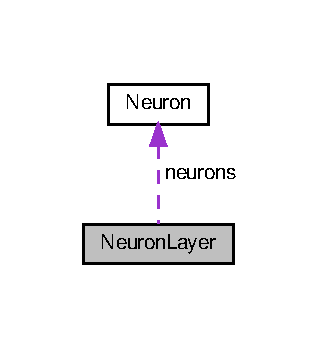
\includegraphics[width=154pt]{structNeuronLayer__coll__graph}
\end{center}
\end{figure}
\subsection*{Data Fields}
\begin{DoxyCompactItemize}
\item 
\hyperlink{structNeuron}{Neuron} $\ast$$\ast$ \hyperlink{structNeuronLayer_a784ca23934ab18af5f24e6b5388ab777}{neurons}
\item 
int \hyperlink{structNeuronLayer_a5f293e290fbfdde756fe43af034ec421}{num\+\_\+neurons}
\end{DoxyCompactItemize}


\subsection{Detailed Description}
The basic structure of a neuron layer. 

\subsection{Field Documentation}
\mbox{\Hypertarget{structNeuronLayer_a784ca23934ab18af5f24e6b5388ab777}\label{structNeuronLayer_a784ca23934ab18af5f24e6b5388ab777}} 
\index{Neuron\+Layer@{Neuron\+Layer}!neurons@{neurons}}
\index{neurons@{neurons}!Neuron\+Layer@{Neuron\+Layer}}
\subsubsection{\texorpdfstring{neurons}{neurons}}
{\footnotesize\ttfamily \hyperlink{structNeuron}{Neuron}$\ast$$\ast$ Neuron\+Layer\+::neurons}

The array of pointers to neurons which will compound the layer. \mbox{\Hypertarget{structNeuronLayer_a5f293e290fbfdde756fe43af034ec421}\label{structNeuronLayer_a5f293e290fbfdde756fe43af034ec421}} 
\index{Neuron\+Layer@{Neuron\+Layer}!num\+\_\+neurons@{num\+\_\+neurons}}
\index{num\+\_\+neurons@{num\+\_\+neurons}!Neuron\+Layer@{Neuron\+Layer}}
\subsubsection{\texorpdfstring{num\+\_\+neurons}{num\_neurons}}
{\footnotesize\ttfamily int Neuron\+Layer\+::num\+\_\+neurons}

T\+He number of Neurons in this layer. 

The documentation for this struct was generated from the following file\+:\begin{DoxyCompactItemize}
\item 
/home/albert/\+Desktop/\+D\+E\+V/\+H\+P-\/\+A\+N\+N/include/\hyperlink{neuronLayer_8h}{neuron\+Layer.\+h}\end{DoxyCompactItemize}

\chapter{File Documentation}
\hypertarget{activation_8h}{}\section{/home/albert/\+Desktop/\+D\+E\+V/\+H\+P-\/\+A\+N\+N/include/activation.h File Reference}
\label{activation_8h}\index{/home/albert/\+Desktop/\+D\+E\+V/\+H\+P-\/\+A\+N\+N/include/activation.\+h@{/home/albert/\+Desktop/\+D\+E\+V/\+H\+P-\/\+A\+N\+N/include/activation.\+h}}


This header file contains all the implemented activation functions and its derivatives.  


\subsection*{Functions}
\begin{DoxyCompactItemize}
\item 
int \hyperlink{activation_8h_ad2f32904e749841eda6b19a5bdc368e2}{Activation\+Logistic} (double x, double $\ast$y, void $\ast$prm)
\begin{DoxyCompactList}\small\item\em Logistic function. \end{DoxyCompactList}\item 
int \hyperlink{activation_8h_a68efe10566ce071243c9031d0a74ec29}{Derivative\+Logistic} (double x, double $\ast$y, void $\ast$prm)
\begin{DoxyCompactList}\small\item\em Derivative of Logistic function. \end{DoxyCompactList}\end{DoxyCompactItemize}


\subsection{Detailed Description}
This header file contains all the implemented activation functions and its derivatives. 

In order to difference both tyes of functions, we have set the following nomenclature\+:
\begin{DoxyItemize}
\item Activation\$\+F\+U\+NC\+: implementation of the activation function F\+U\+NC.
\item Derivative\$\+F\+U\+NC\+: implementation of the derivative of the activation function F\+U\+NC.
\end{DoxyItemize}

All the functions will have 3 main parameters\+:
\begin{DoxyItemize}
\item x\+: the input value
\item y\+: the output value
\item (void$\ast$) prm\+: an array of parameters
\end{DoxyItemize}

The output of the functions will be 1 if no error has happened.

Up to now, the implemented activation functions are\+:
\begin{DoxyItemize}
\item Logistic 
\end{DoxyItemize}

\subsection{Function Documentation}
\mbox{\Hypertarget{activation_8h_ad2f32904e749841eda6b19a5bdc368e2}\label{activation_8h_ad2f32904e749841eda6b19a5bdc368e2}} 
\index{activation.\+h@{activation.\+h}!Activation\+Logistic@{Activation\+Logistic}}
\index{Activation\+Logistic@{Activation\+Logistic}!activation.\+h@{activation.\+h}}
\subsubsection{\texorpdfstring{Activation\+Logistic()}{ActivationLogistic()}}
{\footnotesize\ttfamily int Activation\+Logistic (\begin{DoxyParamCaption}\item[{double}]{x,  }\item[{double $\ast$}]{y,  }\item[{void $\ast$}]{prm }\end{DoxyParamCaption})}



Logistic function. 

The logistic function is defined as\+: \[ f(x) = \frac{1}{1-e^{-x}}. \] 
\begin{DoxyParams}{Parameters}
{\em x} & Input value. \\
\hline
{\em y} & Pointer to the output value of the function. \\
\hline
{\em prm} & Pointer to parameters. Insert N\+U\+LL pointer. \\
\hline
\end{DoxyParams}
\begin{DoxyReturn}{Returns}
1 if nothing wrong happenes, 0 otherwise. 
\end{DoxyReturn}
\mbox{\Hypertarget{activation_8h_a68efe10566ce071243c9031d0a74ec29}\label{activation_8h_a68efe10566ce071243c9031d0a74ec29}} 
\index{activation.\+h@{activation.\+h}!Derivative\+Logistic@{Derivative\+Logistic}}
\index{Derivative\+Logistic@{Derivative\+Logistic}!activation.\+h@{activation.\+h}}
\subsubsection{\texorpdfstring{Derivative\+Logistic()}{DerivativeLogistic()}}
{\footnotesize\ttfamily int Derivative\+Logistic (\begin{DoxyParamCaption}\item[{double}]{x,  }\item[{double $\ast$}]{y,  }\item[{void $\ast$}]{prm }\end{DoxyParamCaption})}



Derivative of Logistic function. 

Given the logistic function $f(x)$, its derivative is computed as $f'(x)=f(x)(1-f(x))$. 
\begin{DoxyParams}{Parameters}
{\em x} & Input value. \\
\hline
{\em y} & Pointer to the output value of the function. \\
\hline
{\em prm} & Pointer to parameters. Insert N\+U\+LL pointer. \\
\hline
\end{DoxyParams}
\begin{DoxyReturn}{Returns}
1 if Nothing wrong happenes, 0 otherwise. 
\end{DoxyReturn}

\hypertarget{neuron_8h}{}\section{/home/albert/\+Desktop/\+D\+E\+V/\+H\+P-\/\+A\+N\+N/include/neuron.h File Reference}
\label{neuron_8h}\index{/home/albert/\+Desktop/\+D\+E\+V/\+H\+P-\/\+A\+N\+N/include/neuron.\+h@{/home/albert/\+Desktop/\+D\+E\+V/\+H\+P-\/\+A\+N\+N/include/neuron.\+h}}


This header file contains the structure of the \hyperlink{structNeuron}{Neuron} and its basic functions.  


This graph shows which files directly or indirectly include this file\+:\nopagebreak
\begin{figure}[H]
\begin{center}
\leavevmode
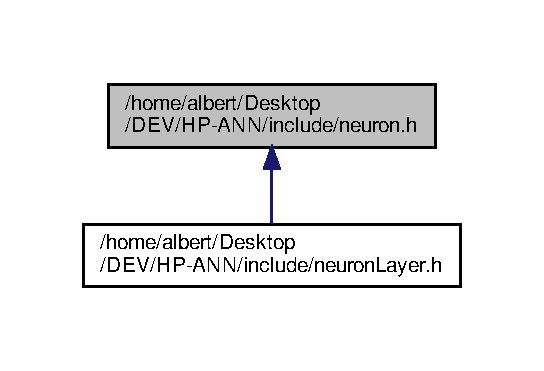
\includegraphics[width=261pt]{neuron_8h__dep__incl}
\end{center}
\end{figure}
\subsection*{Data Structures}
\begin{DoxyCompactItemize}
\item 
struct \hyperlink{structNeuron}{Neuron}
\begin{DoxyCompactList}\small\item\em The basic structure of a \hyperlink{structNeuron}{Neuron}. \end{DoxyCompactList}\end{DoxyCompactItemize}
\subsection*{Functions}
\begin{DoxyCompactItemize}
\item 
\hyperlink{structNeuron}{Neuron} $\ast$ \hyperlink{neuron_8h_a43a7f8eaba97fda5a0b17535c4b44a20}{create\+Neuron} (double value, double act\+Val)
\item 
void \hyperlink{neuron_8h_ad2eb23bf0a3e63a9261ba553150a2550}{free\+Neuron} (\hyperlink{structNeuron}{Neuron} $\ast$neuron)
\begin{DoxyCompactList}\small\item\em Function to destroy a given neuron. \end{DoxyCompactList}\item 
void \hyperlink{neuron_8h_a5d3c7fe3b5184be5af72e1ac30f1938a}{set\+Value\+Neuron} (\hyperlink{structNeuron}{Neuron} $\ast$neuron, double value)
\begin{DoxyCompactList}\small\item\em Function to set a new value to a given \hyperlink{structNeuron}{Neuron}. \end{DoxyCompactList}\item 
void \hyperlink{neuron_8h_af67de49f3e4ac24bff9085106ee8599c}{activate\+Neuron} (\hyperlink{structNeuron}{Neuron} $\ast$neuron, int($\ast$f)(double x, double $\ast$y, void $\ast$prm), void $\ast$prm)
\begin{DoxyCompactList}\small\item\em Function to set an activation value given an activation function. \end{DoxyCompactList}\end{DoxyCompactItemize}


\subsection{Detailed Description}
This header file contains the structure of the \hyperlink{structNeuron}{Neuron} and its basic functions. 



\subsection{Function Documentation}
\mbox{\Hypertarget{neuron_8h_af67de49f3e4ac24bff9085106ee8599c}\label{neuron_8h_af67de49f3e4ac24bff9085106ee8599c}} 
\index{neuron.\+h@{neuron.\+h}!activate\+Neuron@{activate\+Neuron}}
\index{activate\+Neuron@{activate\+Neuron}!neuron.\+h@{neuron.\+h}}
\subsubsection{\texorpdfstring{activate\+Neuron()}{activateNeuron()}}
{\footnotesize\ttfamily void activate\+Neuron (\begin{DoxyParamCaption}\item[{\hyperlink{structNeuron}{Neuron} $\ast$}]{neuron,  }\item[{int($\ast$)(double x, double $\ast$y, void $\ast$prm)}]{f,  }\item[{void $\ast$}]{prm }\end{DoxyParamCaption})}



Function to set an activation value given an activation function. 


\begin{DoxyParams}{Parameters}
{\em neuron} & The neuron we want to activate. \\
\hline
{\em f} & The activation function we will use. \\
\hline
{\em prm} & Parameters that might have the activation function. \\
\hline
\end{DoxyParams}
\mbox{\Hypertarget{neuron_8h_a43a7f8eaba97fda5a0b17535c4b44a20}\label{neuron_8h_a43a7f8eaba97fda5a0b17535c4b44a20}} 
\index{neuron.\+h@{neuron.\+h}!create\+Neuron@{create\+Neuron}}
\index{create\+Neuron@{create\+Neuron}!neuron.\+h@{neuron.\+h}}
\subsubsection{\texorpdfstring{create\+Neuron()}{createNeuron()}}
{\footnotesize\ttfamily \hyperlink{structNeuron}{Neuron}$\ast$ create\+Neuron (\begin{DoxyParamCaption}\item[{double}]{value,  }\item[{double}]{act\+Val }\end{DoxyParamCaption})}

Function to create a new neuron. It allocates The necessary memory to create a neuron. 
\begin{DoxyParams}{Parameters}
{\em value} & The value to be stored by the neuron. \\
\hline
{\em act\+Val} & The activation value to be stored by the neuron. \\
\hline
\end{DoxyParams}
\mbox{\Hypertarget{neuron_8h_ad2eb23bf0a3e63a9261ba553150a2550}\label{neuron_8h_ad2eb23bf0a3e63a9261ba553150a2550}} 
\index{neuron.\+h@{neuron.\+h}!free\+Neuron@{free\+Neuron}}
\index{free\+Neuron@{free\+Neuron}!neuron.\+h@{neuron.\+h}}
\subsubsection{\texorpdfstring{free\+Neuron()}{freeNeuron()}}
{\footnotesize\ttfamily void free\+Neuron (\begin{DoxyParamCaption}\item[{\hyperlink{structNeuron}{Neuron} $\ast$}]{neuron }\end{DoxyParamCaption})}



Function to destroy a given neuron. 


\begin{DoxyParams}{Parameters}
{\em neuron} & The neuron to delete. \\
\hline
\end{DoxyParams}
\mbox{\Hypertarget{neuron_8h_a5d3c7fe3b5184be5af72e1ac30f1938a}\label{neuron_8h_a5d3c7fe3b5184be5af72e1ac30f1938a}} 
\index{neuron.\+h@{neuron.\+h}!set\+Value\+Neuron@{set\+Value\+Neuron}}
\index{set\+Value\+Neuron@{set\+Value\+Neuron}!neuron.\+h@{neuron.\+h}}
\subsubsection{\texorpdfstring{set\+Value\+Neuron()}{setValueNeuron()}}
{\footnotesize\ttfamily void set\+Value\+Neuron (\begin{DoxyParamCaption}\item[{\hyperlink{structNeuron}{Neuron} $\ast$}]{neuron,  }\item[{double}]{value }\end{DoxyParamCaption})}



Function to set a new value to a given \hyperlink{structNeuron}{Neuron}. 


\begin{DoxyParams}{Parameters}
{\em neuron} & The neuron which will have a new value. \\
\hline
{\em value} & The new value of the neuron. \\
\hline
\end{DoxyParams}

\hypertarget{neuronLayer_8h}{}\section{/home/albert/\+Desktop/\+D\+E\+V/\+H\+P-\/\+A\+N\+N/include/neuron\+Layer.h File Reference}
\label{neuronLayer_8h}\index{/home/albert/\+Desktop/\+D\+E\+V/\+H\+P-\/\+A\+N\+N/include/neuron\+Layer.\+h@{/home/albert/\+Desktop/\+D\+E\+V/\+H\+P-\/\+A\+N\+N/include/neuron\+Layer.\+h}}


This header file contains the structure of the \hyperlink{structNeuronLayer}{Neuron\+Layer} and its basic functions.  


{\ttfamily \#include \char`\"{}../include/neuron.\+h\char`\"{}}\newline
Include dependency graph for neuron\+Layer.\+h\+:\nopagebreak
\begin{figure}[H]
\begin{center}
\leavevmode
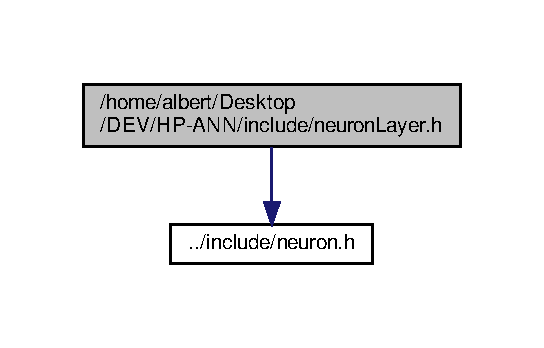
\includegraphics[width=261pt]{neuronLayer_8h__incl}
\end{center}
\end{figure}
\subsection*{Data Structures}
\begin{DoxyCompactItemize}
\item 
struct \hyperlink{structNeuronLayer}{Neuron\+Layer}
\begin{DoxyCompactList}\small\item\em The basic structure of a neuron layer. \end{DoxyCompactList}\end{DoxyCompactItemize}
\subsection*{Functions}
\begin{DoxyCompactItemize}
\item 
\hyperlink{structNeuronLayer}{Neuron\+Layer} $\ast$ \hyperlink{neuronLayer_8h_ae036ca8d6dedad48e380e24e0ae3d4f9}{create\+Neuron\+Layer} (int num, double $\ast$value, double $\ast$act\+Val)
\begin{DoxyCompactList}\small\item\em Function to create a new \hyperlink{structNeuronLayer}{Neuron\+Layer}. It allocates the necessary memory to create a neuron layer. \end{DoxyCompactList}\item 
void \hyperlink{neuronLayer_8h_a6b62f439ffc6fca1dcdae539d4ababe8}{free\+Neuron\+Layer} (\hyperlink{structNeuronLayer}{Neuron\+Layer} $\ast$nl)
\begin{DoxyCompactList}\small\item\em Function to destroy a given neuron layer. \end{DoxyCompactList}\item 
void \hyperlink{neuronLayer_8h_ae302266895a38caffecd3f04690d27d9}{set\+Value\+Neuron\+Layer} (\hyperlink{structNeuronLayer}{Neuron\+Layer} $\ast$nl, double $\ast$value)
\begin{DoxyCompactList}\small\item\em Function to set a new value to a given \hyperlink{structNeuronLayer}{Neuron\+Layer}. \end{DoxyCompactList}\item 
void \hyperlink{neuronLayer_8h_ac73ebccd77dfe3f208219e8a222eb1a5}{activate\+Neuron\+Layer} (\hyperlink{structNeuronLayer}{Neuron\+Layer} $\ast$nl, int($\ast$f)(double x, double $\ast$y, void $\ast$prm), void $\ast$prm)
\begin{DoxyCompactList}\small\item\em Function to set an activation value given an activation function for a Neural Layer. \end{DoxyCompactList}\end{DoxyCompactItemize}


\subsection{Detailed Description}
This header file contains the structure of the \hyperlink{structNeuronLayer}{Neuron\+Layer} and its basic functions. 



\subsection{Function Documentation}
\mbox{\Hypertarget{neuronLayer_8h_ac73ebccd77dfe3f208219e8a222eb1a5}\label{neuronLayer_8h_ac73ebccd77dfe3f208219e8a222eb1a5}} 
\index{neuron\+Layer.\+h@{neuron\+Layer.\+h}!activate\+Neuron\+Layer@{activate\+Neuron\+Layer}}
\index{activate\+Neuron\+Layer@{activate\+Neuron\+Layer}!neuron\+Layer.\+h@{neuron\+Layer.\+h}}
\subsubsection{\texorpdfstring{activate\+Neuron\+Layer()}{activateNeuronLayer()}}
{\footnotesize\ttfamily void activate\+Neuron\+Layer (\begin{DoxyParamCaption}\item[{\hyperlink{structNeuronLayer}{Neuron\+Layer} $\ast$}]{nl,  }\item[{int($\ast$)(double x, double $\ast$y, void $\ast$prm)}]{f,  }\item[{void $\ast$}]{prm }\end{DoxyParamCaption})}



Function to set an activation value given an activation function for a Neural Layer. 


\begin{DoxyParams}{Parameters}
{\em nl} & The \hyperlink{structNeuron}{Neuron} Layer we want to activate. \\
\hline
{\em f} & The activation function we will use. \\
\hline
{\em prm} & Parameters that might have the activation function. \\
\hline
\end{DoxyParams}
\mbox{\Hypertarget{neuronLayer_8h_ae036ca8d6dedad48e380e24e0ae3d4f9}\label{neuronLayer_8h_ae036ca8d6dedad48e380e24e0ae3d4f9}} 
\index{neuron\+Layer.\+h@{neuron\+Layer.\+h}!create\+Neuron\+Layer@{create\+Neuron\+Layer}}
\index{create\+Neuron\+Layer@{create\+Neuron\+Layer}!neuron\+Layer.\+h@{neuron\+Layer.\+h}}
\subsubsection{\texorpdfstring{create\+Neuron\+Layer()}{createNeuronLayer()}}
{\footnotesize\ttfamily \hyperlink{structNeuronLayer}{Neuron\+Layer}$\ast$ create\+Neuron\+Layer (\begin{DoxyParamCaption}\item[{int}]{num,  }\item[{double $\ast$}]{value,  }\item[{double $\ast$}]{act\+Val }\end{DoxyParamCaption})}



Function to create a new \hyperlink{structNeuronLayer}{Neuron\+Layer}. It allocates the necessary memory to create a neuron layer. 


\begin{DoxyParams}{Parameters}
{\em num} & number of neurons of this layer. \\
\hline
{\em value} & the values to be stored by the neurons. \\
\hline
{\em act\+Val} & the activation values to be stored by the neurons. \\
\hline
\end{DoxyParams}
\mbox{\Hypertarget{neuronLayer_8h_a6b62f439ffc6fca1dcdae539d4ababe8}\label{neuronLayer_8h_a6b62f439ffc6fca1dcdae539d4ababe8}} 
\index{neuron\+Layer.\+h@{neuron\+Layer.\+h}!free\+Neuron\+Layer@{free\+Neuron\+Layer}}
\index{free\+Neuron\+Layer@{free\+Neuron\+Layer}!neuron\+Layer.\+h@{neuron\+Layer.\+h}}
\subsubsection{\texorpdfstring{free\+Neuron\+Layer()}{freeNeuronLayer()}}
{\footnotesize\ttfamily void free\+Neuron\+Layer (\begin{DoxyParamCaption}\item[{\hyperlink{structNeuronLayer}{Neuron\+Layer} $\ast$}]{nl }\end{DoxyParamCaption})}



Function to destroy a given neuron layer. 


\begin{DoxyParams}{Parameters}
{\em nl} & The neural layer to destroy. \\
\hline
\end{DoxyParams}
\mbox{\Hypertarget{neuronLayer_8h_ae302266895a38caffecd3f04690d27d9}\label{neuronLayer_8h_ae302266895a38caffecd3f04690d27d9}} 
\index{neuron\+Layer.\+h@{neuron\+Layer.\+h}!set\+Value\+Neuron\+Layer@{set\+Value\+Neuron\+Layer}}
\index{set\+Value\+Neuron\+Layer@{set\+Value\+Neuron\+Layer}!neuron\+Layer.\+h@{neuron\+Layer.\+h}}
\subsubsection{\texorpdfstring{set\+Value\+Neuron\+Layer()}{setValueNeuronLayer()}}
{\footnotesize\ttfamily void set\+Value\+Neuron\+Layer (\begin{DoxyParamCaption}\item[{\hyperlink{structNeuronLayer}{Neuron\+Layer} $\ast$}]{nl,  }\item[{double $\ast$}]{value }\end{DoxyParamCaption})}



Function to set a new value to a given \hyperlink{structNeuronLayer}{Neuron\+Layer}. 


\begin{DoxyParams}{Parameters}
{\em nl} & The neural layer to set new values. \\
\hline
{\em value} & The array of new values (must have the same length as the neural layer). \\
\hline
\end{DoxyParams}

%--- End generated contents ---

% Index
\backmatter
\newpage
\phantomsection
\clearemptydoublepage
\addcontentsline{toc}{chapter}{Index}
\printindex

\end{document}
